%% LyX 2.2.2 created this file.  For more info, see http://www.lyx.org/.
%% Do not edit unless you really know what you are doing.
\documentclass[a4paper,twoside,british,cleardoublepage=empty,BCOR15mm,DIV12]{scrreprt}
\usepackage{amsmath}
\usepackage{tgtermes}
\usepackage{tgheros}
\usepackage{tgcursor}
\usepackage{newtxmath}
\usepackage[T1]{fontenc}
\usepackage[utf8]{inputenc}
\usepackage{babel}
\usepackage{graphicx}
\usepackage[unicode=true,pdfusetitle,
 bookmarks=true,bookmarksnumbered=false,bookmarksopen=false,
 breaklinks=false,pdfborder={0 0 1},backref=false,colorlinks=false]
 {hyperref}

\makeatletter

%%%%%%%%%%%%%%%%%%%%%%%%%%%%%% LyX specific LaTeX commands.
\pdfpageheight\paperheight
\pdfpagewidth\paperwidth

\newcommand{\noun}[1]{\textsc{#1}}
%% Because html converters don't know tabularnewline
\providecommand{\tabularnewline}{\\}

%%%%%%%%%%%%%%%%%%%%%%%%%%%%%% User specified LaTeX commands.
%<-------------------------------společná nastavení------------------------------>
\usepackage[numbers,sort&compress]{natbib} %balíček pro citace literatury  
\usepackage{algorithmic}
\usepackage{color}%kvůli barvám ČVUT
\newcommand{\BibTeX}{{\sc Bib}\TeX}%BibTeX logo
\usepackage{multicol}
\usepackage[overload]{textcase}



%<-----------------------------volání stylů----------------------------------------->
% (znak % je označení komentáře: co je za ním, není aktivní)

%<--------matematické písmo--------------------------------------->

%\usepackage[helvet]{packages/sfmath}%matematika ala helvetica



%<------------------------------záhlaví stránek------------------------------------>
%\usepackage{packages/bc-headings}
\usepackage{packages/bc-fancyhdr}

%<------------------------------hlavičky kapitol------------------------------------>
%\usepackage{packages/bc-neueskapitel}
\usepackage{packages/bc-fancychap}

\makeatother

\usepackage{listings}
\renewcommand{\lstlistingname}{\inputencoding{latin9}Listing}

\begin{document}
~\thispagestyle{empty}\begin{center}\pagenumbering{arabic}\vspace{10mm}

\textsf{\textsc{\noun{\LARGE{}Czech Technical University in Prague}}}\\
\vspace{0.5em}
\textsf{\textsc{\noun{\LARGE{}Faculty of Electrical Engineering}}}\\
\vspace*{1em}
\textsf{\textsc{\noun{\Large{}Department of Cybernetics}}}\vspace{15mm}


\includegraphics[width=0.3\textwidth]{obrazky/lev}\vspace{15mm}

\textsf{\huge{}MASTER'S THESIS}{\huge \par}

\vspace{15mm}

\textsf{\LARGE{}3D map estimation from a single RGB image}{\LARGE \par}

\vspace{10mm}

\end{center} 

\vspace*{\fill}

\vspace{10mm}

\begin{description}
\item [{{\large{}Author:}}] \noindent \textsf{\large{}Bc. Matěj Račinský}{\large \par}
\item [{{\large{}Thesis~supervisor:}}] \noindent {\large{}doc. Ing. Karel
Zimmermann, Ph.D.\hfill{}}\textsf{\large{}In Prague, May 2018}{\large \par}
\end{description}
\cleardoublepage{}\thispagestyle{empty}~

{\small{}\ }{\small \par}

\noindent {\small{}\vfill{}
 % nastavuje dynamické umístění následujícího textu do spodní části stránky
~}{\small \par}

\subparagraph*{Author statement for thegraduate thesis: \protect \\
}

I declare that the presented work was developed independently and
that I have listed all the sources of information used within it in
accordance with the methodical instructions for observing the ethical
principles in the presentation of university theses. 

{\small{}\bigskip{}
}\noindent {\small{} Prague, date }\_\_\_\_\_\_\_\_{\small{}\hspace{\fill}$\overline{\textrm{~~~~~~~~~signature~~~}}$}\\
{\small{} % doplňte patřičné datum, jméno a příjmení
}{\small \par}

{\small{}%%%   Výtisk pak na tomto míste nezapomeňte PODEPSAT!
%%%                                         *********
}{\small \par}

\cleardoublepage{}

{\small{}\thispagestyle{plain} }{\small \par}

{\small{}%\setcounter{page}{3} % nastavení číslování stránek
}{\small \par}

\noindent {\small{}~\vfill{}
}{\small \par}
\begin{description}
\item [{{\small{}Název~práce:}}] \noindent {\small{}Odhad 3D mapy z jednoho
RGB obrazu}{\small \par}
\item [{{\small{}Autor:}}] \noindent {\small{}Bc. Matěj Račinský}{\small \par}
\item [{{\small{}Katedra~(ústav):}}] \noindent Kate{\small{}dra kybernetiky}{\small \par}
\item [{{\small{}Vedoucí~bakalářské~práce:}}] \noindent {\large{}doc.
Ing. Karel Zimmermann, Ph.D.}{\large \par}
\item [{{\small{}e-mail~vedoucího:}}] \noindent {\small{}zimmerk@fel.cvut.cz}\\
{\small \par}
\item [{{\small{}Abstrakt}}] \noindent Tato práce se zabývá využitím virtuálních
světů z počítačových her jakožto zdroje dat pro strojové učení, a
odhadem voxelové mapy z jednoho RGB obrázku za pomoci hlubokého učení.
Tato práce zahrnuje skripty pro napojení se na PC hru GTA V a sběr
dat z ní pro tvorbu automaticky anotovaných datasetů, a implementaci
hluboké neuronové sítě v TensorFlow. 
\item [{{\small{}Klíčová~slova:}}] \noindent {\small{}Deep learning, Machine
learning, GTA V, virtual world, depth estimation, voxelmap estimation,
RAGE}\\
{\small \par}
\item [{\rule[0.5ex]{1\linewidth}{1pt}}]~{\small \par}
\item [{{\small{}Title:}}] \noindent {\small{}3D map estimation from a
single RGB image}{\small \par}
\item [{{\small{}Author:}}] \noindent {\small{}Bc. Matěj Račinský}{\small \par}
\item [{{\small{}Department:}}] \noindent {\small{}Department of Cybernetics}{\small \par}
\item [{{\small{}Supervisor:}}] \noindent {\large{}doc. Ing. Karel Zimmermann,
Ph.D.}{\large \par}
\item [{{\small{}Supervisor's~e-mail~address:}}] \noindent {\small{}zimmerk@fel.cvut.cz}\\
{\small \par}
\item [{{\small{}Abstract}}] \noindent In this thesis we explore virtual
worlds used as datasoutce for machine learning and voxelmap estimation
from single RGB image with deep learning. This thesis describes principles
and omplementation of hooking into GTA V and gathering data from it
to create automatically annotated dataset, and implementation of deep
neural network in TensorFlow.
\item [{{\small{}Keywords:}}] \noindent {\small{}Deep learning, Machine
learning, GTA V, virtual world, depth estimation, voxelmap estimation,
RAGE}{\small \par}
\end{description}
{\small{}\tableofcontents{}% vkládá automaticky generovaný obsah dokumentu
}{\small \par}

\chapter[Introduction]{Introduction}

This thesis aims to solve two problems. The first problem is the lengthy
and slow process of manual dataset creation and annotation, and the
second problem is voxelmap estimation from single RGB image. Due to
increasing interest in synthetic datasets, this thesis aims to be
the documentation for using GTA V as simulator for creation of synthetic
datasets.

\section{Problems with machine learning datasets}

In recent years, both machine learning and deep learning has experienced
great progress in many fields. Deep learning has outperformed many
other machine learning approaches by using deep, high-capacity models
trained on large datasets. Especially in the field of computer vision,
neural networks achieve state of the art results in most of the tasks.
Many tasks in computer vision are the first where deep neural networks
achieve state of the art results before being used in other fields,
and in this field deeper and deeper architectures are being proposed
earlier than in other fields. 

With larger amount of parameters, the need for large datasets is growing,
with currect datasets unable to cover the need for annotated data.

Data has proven to be limiting factor in many computer vision tasks.
The main problem is that manual data annotation is exhausting, time-consuming
and costly. That is even more significant for pixel-wise annotation
which is crucial for tasks of semantic segmentation. Pixel-wise annotated
datasets are orders of magnitude smaller than image classification
datasets. This is sometimes called ``curse of dataset annotation''\cite{semantic-instance-annotation},
because more detailed semantic labeling leads to smaller size of dataset. 

Many novel neural network architectures are being proposed every year
because of increasing computing power. With growing capacity and number
of parameters in these new models, there is need for bigger and bigger
datasets for training. 

Automatic data gathering and automatic data annotation could potentially
solve these problems of lack of datasets in many computer vision and
related tasks.

\section{Gaming industry to the rescue}

In last decades, gaming industry has grown hugely and expanded from
small and specific community into public society and became mainsteam
industy. 

The gaming industry became big driving force in many fields, and indirectly
influenced even machine learning. 

The mainsteam model of gaming is on personal computers, where each
player has his own gaming PC, along with console gaming. Thanks to
ever-growing number of players, lots of money got into industry and
the growing demand for better graphics in games led to big improvements
in both software-computer graphics and hardware-graphics cards. With
lots of money being invested by players in their PCs, GPU manufacturers
were able to deliver more powerful GPUs every year and we can see
exponential growth of GPU computational power\cite{high-performance-gpu}.

Big companies in gaming industry have enough resources to develop
the state of the art real-time computer graphics, which can we see
in their products, AAA games with graphics very near to reality. 

Recent papers\cite{playing-for-data,driving-in-matrix} show that
we can use screenshots from PC games to obtain large automatically
or semi-automatically annotated datasets, which improve learning,
allow us to outperform same models trained only on real data and achieve
state of the art results.

\chapter{Related work}

\cite{playing-for-data} used GTA V to obtain screenshots and performed
semi-automated pixel-wise semantic segmentation. Although the process
was not fully automatic, the annotation speed per image was drastically
increased, being 771 times faster than fine per-image annotation of
Cityscapes \cite{cityscapes} and 514 times faster than per-image
annotation of CamVid\cite{camvid}. They extracted 24 966 images from
game GTA V, which is roughly two orders of magnitude larger than CanVid
and three orders of magnitude larger than semantic annotations for
KITTI dataset. They trained the prediction module of Yu and Koltun\cite{kolthun-dilation}
and by using on $\frac{1}{3}$of the CamVid training set (which is
) and all 24 966 GTA V screenshots, they outperformed same model trained
on whole CamVid training dataset.

For images extraction, they use RenderDoc\cite{renderdoc}, stand-alone
graphics debugger. It intercepts the communication between the game
and the GPU and allows to gather screenshots. It's advantage is that
it can be used for different games, allowing to gather datasets in
various environments.

\cite{driving-in-matrix} use GTA V screenshots, depth and stencil
buffer to produce car images and automatically calculate their bounding
boxes. 

On these generated data, they trained Faster R-CNN\cite{faster-r-cnn}
only of screenshots from the GTA V game, using up to 200 000 screenshots,
which is one order of magnitude bigger than Cityscapes dataset. Using
only screenshots for training, they outperformed same architecture
trained on Cityscapes, evaluating on KITTI dataset. They developed
their own GTA V mod\ref{sec:GTA-V-modding} to hook into GPU calls
and gather screenshots from here. 

\chapter{Transforming GTA V into the State of the Art simulator}

In this thesis, Grand Theft Auto V (GTA V) game is used for creating
synthetic, nearly photo-realistic dataset. 

\section{GTA V introduction}

GTA V is action-adventure open-world video game developed by Rockstar
North and published by Rockstar Games. The game was released on 17.9.2013
for Playstation 3 and Xbox 360\cite{gta-release} , in 18.11.2014
for PS4 and Xbox One and in 14.4.2015 it was released on PC, Windows\cite{gta-release-pc}.

The game is based on proprietary game engine, called \label{rage}RAGE
(Rockstar Advanced Game Engine)\cite{gta-5-rage}, which is used as
a base for most of Rockstar Games products. 

Till the release on Microsoft, Windows, it has been in development
for 5 years with approximate 1000-person team\cite{gta-interview-studio}.
The world of GTA V was modelled on Los Angeles\cite{gta-v-interview}
and other areas of Southen California, with road networks respecting
design od Los Angeles map. 

As could be expected from AAA game like GTA V, motion capture was
used to character's both body and facial movements. 

There are several reasons why GTA V is better for dataset creationg
than other games. To use a game for dataset creation, we have multiple
requirements. The graphics of the game must be near photorealistic,
since we try to to use it instead of photos for computer vision tasks.
This disqualifies most of games, and leaves us only with AAA games
produced by big companies and few other games with State of the Art
graphics. 

The other requirement is opssibility of good-enough way to interact
with the game programatically. Usually we want to setup at least part
of the environment before gathering data. This part heavily depends
on community around the particular game.

In gaming subculture, there are communities where people specialize
in reverse-engineering of games and development of modifications to
these games. These people are called modders or mod developers, and
these unofficial modifications and extension of games are called mods.
For few games, developers welcome this kind of activity and sometimes
they even release tools to ease the game modding. In most cases, the
game developers simply don't care and in few cases, they actively
fight against the reverse-engineering and modding. 

The GTA V is second case, where Rockstar Games does not actively try
to prevent the reverse-engineering, but they don't release any tools
to ease it, either. This results in cyclic process of Rockstar Games
releasing new version of game, including backward compatibility (BC)
breaks, and community reverse engineering the new version and adjusting
their mods to work with the new version.

The modding community around the GTA V is based mostly on community
around GTA IV, which was previous big game produced by Rockstar Games.
So many tools are just GTA IV based and only modified to work with
GTA V. Luckily, the community is large and productive, so we have
many mods and many function in GTA V reverse-engineered and thus prepared
for programatic interactions.

\section{Automotive Simulators}

Currently, there are some opensorce simulation platforms for automotive
industry which could be theoretically used for creating synthetic
datasets. But compared to AAA games like GTA V, they have much less
resources and much less customers to finance the development. In result,
simulators have worse graphics than AAA games and NPC (non playable
characters) don't have as sophisticated behaviour. In GTA V, drivers
mostly follow traffic regulations, traffic lights and traffic lanes,
which leafs to very realistic environment better than simulators can
provide.

\section{\label{sec:GTA-V-modding}GTA V modding ecosystem}

Although the modding community is quite big, as it is in lots of opensource
communities, essential part of community depends on one person. Here,
it is Alexader Blade. In his free time, he reverse-engineered big
part of GTA V and developed ScriptHookV\cite{scripthookv-gtaforums},
library enabling to perform native calls into GTA V in C++ and develop
GTA V mods in C++. Currently, more people in community participates
in reverse-engineering and they share their knowledge in GTA forum
thread\cite{nativedb-research}.

List of all reverse-engineered native functions is kept in following
list \cite{nativedb}. Assumingly, GTA V contains \textasciitilde{}5200
natives. There is no original native name list of functions in GTA
V, name hashes are used instead. During reverse-engineering ande game
decompilation, \textasciitilde{}2600 native names were discovered
using bruteforce and manual checking afterwards. For these functions,
number of parameters and returns of these calls are also known. In
the native functions list, for big part of functions we know their
name, signature and how do they affect the game. The rest remains
to be discovered yet.

When new version of game is released, in few days to weeks, new version
of ScriptHookV is released, fixing BC breaks.

Other heavily used mod in community is ScriptHookDotNet2, which is
built atop of ScriptHookV and creates bridge between C\# language
and ScriptHookV, effectively allowing to write GTA V mods in C\#.
It is availabe as open-source \cite{scripthookvdotnet}. Along with
creating bridge between C\# and GTA V, it wraps most used native calls
into classes, leveraging object-oriented paradigm for mod development
using getters and setters as proxies for native calls. 

Next notable mod is NativeUI\cite{nativeui}. It renders windows atop
of GTA V GUI and allows us to define custom control panels for manipulating
custom functionality in other mods. 

Unlike most of other mods, these three mods act more as a framework
for mod development. 

Since GTA V is a game, it requires human interaction. For simulator-like
behavior we would want the car to drive autonomously to crawl data
without human interaction. This can be done using VAutodrive\cite{vautodrive}.
This allows us to use NPC automatic behaviour patterns for main player,
letting the player randomly wander the world, even in car, without
need of human assistance during crawling. Unfortunately, this package
is not open-source.

Generally, the community is not united in their view on opensource.
Some mods are available open-source on github. Other mods are being
distributed only as compiled binaries\cite{gta-5-mods}. Lots of modders
develop mostly by trial and error, and no comprehensive documentation
for mod development is available, unfortunately. There are some tutorials
\cite{gta-5-mod-tutorial}, but they are far from complete and provide
only basic knowledge, leavin reader without deeper understanding of
underlying principles.

Modders mostly meet online on few GTA forums, where they exchange
knowledge \cite{gta-forums,gta-5-mods-forum}. Github or StackOverflow,
which are biggest information sources for usual software development,
are not used much in GTA modding community. Due to this fact, these
forums, along with source code of open-source mods comprise knowledge-base
of mod development.

\section{Simulation environment and development stack}

In this thesis, I use mod based on \cite{driving-in-matrix} but enhanced
to gain more control of the game. Also, the mod in 

In later text, I'll refer to some GTA V native functions or data structures
which are output of GTA V native functions. To be consistent and to
help understanding, I will use function names from native function
list \cite{nativedb}.

\section{GTA V native API and provided data}

\section{Reverse-engineering the RAGE rendering pipeline}

As mentioned above\ref{rage}, GTA V uses proprietary game engine,
Rockstar Advanced Game Engine (RAGE). The basic premise of rendering
pipeline is same as in well known graphics engines like OpenGL. The
pipeline is shown in figure \ref{fig:Visualization-pipeline}. Following
section will be discussing mostly computer graphics related problems.
Due to some terminology inconsistency between computer graphics and
computer vision, all terms used here will be compuer graphics related.
Probably most confusion here could be caused by projection matrix.
In computer vision, projection matrix is projection from 3D to 2D,
the matrix reduces dimension. In computer graphics, all coordinates
are kept in 4D, in homogeneous coordinates as long as possible. Here
the projection matrix prepresents projection from frustum seen by
eye into cuboid space of Normalized Device Coordinates.

\begin{figure}
\begin{centering}
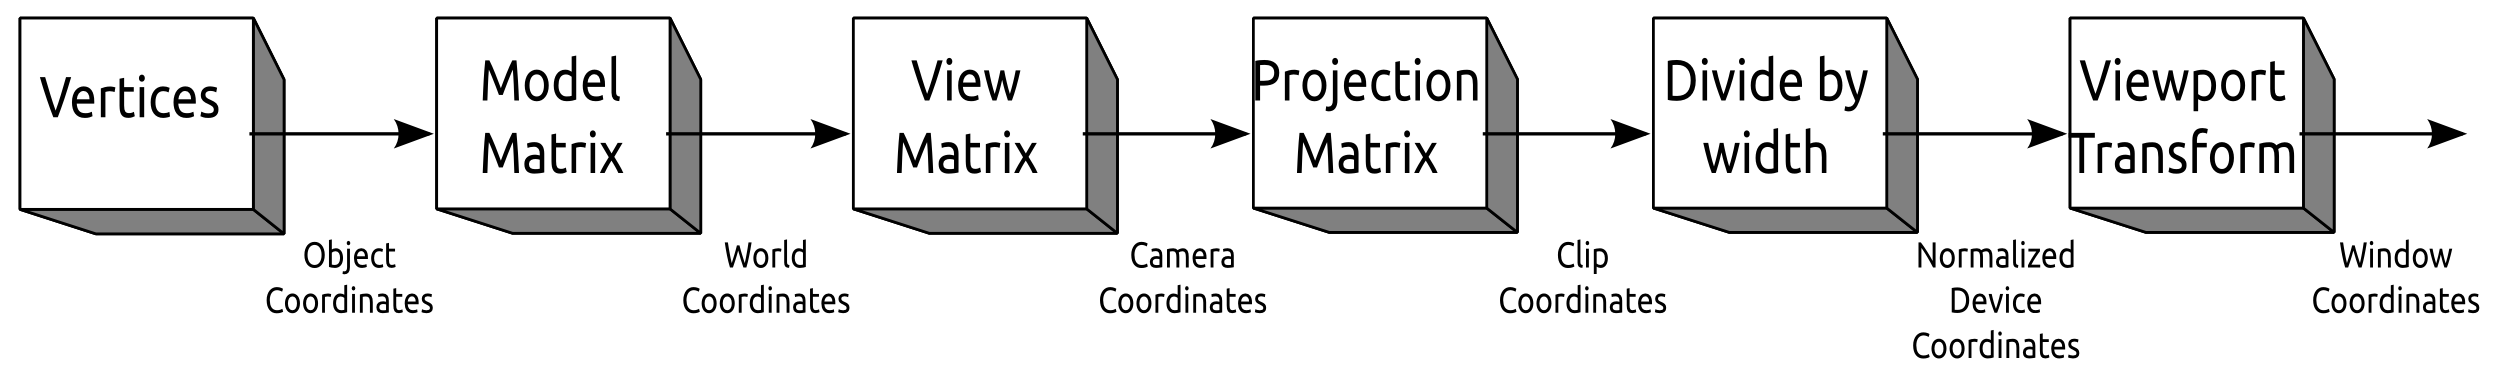
\includegraphics[scale=0.65]{obrazky/transformationPipeline}
\par\end{centering}
\caption{\label{fig:Visualization-pipeline}Rendering pipeline}
\end{figure}
In is part, I will describe some transformations between individual
RAGE coordinate systems. Some points here will have part of name in
lower index. The name of coordinate system will be denoted in upper
index. In RAGE there are 6 coordinate systems.
\begin{center}
\begin{tabular}{|c|c|c|}
\hline 
Name & Abbreviation & Example point $x$\tabularnewline
\hline 
\hline 
Object Coordinates & O & $x^{O}$\tabularnewline
\hline 
World Coordinates & W & $x^{W}$\tabularnewline
\hline 
Camera Coordinates & C & $x^{C}$\tabularnewline
\hline 
Clip Coordinates & L & $x^{L}$\tabularnewline
\hline 
Normalized Device Coordinates & NDC & $x^{NDC}$\tabularnewline
\hline 
Windows Coordinates & P & $x^{P}$\tabularnewline
\hline 
\end{tabular}
\par\end{center}

Most of points we handle in GTA already are in world coordinates. 

But some points, like GAMEPLAY::GET\_MODEL\_DIMENSIONS

$=\begin{pmatrix}x_{max}^{O} & y_{max}^{O} & z_{max}^{O}\end{pmatrix}\begin{pmatrix}x_{min}^{O} & y_{min}^{O} & z_{min}^{O}\end{pmatrix}$
output, are in object coordinates. Transitions between adjacent coordinate
systems will be demonstrated on model dimensions because it is on
the few vectors which are obtained in Object Coordinates and there
is need to project them into Window Coordinates.

\subsection{Object to World Coordinates}

To get world coordinates of model dimensions, we use traditional rigid
body transformation based on ENTITY::GET\_ENTITY\_ROTATION$=\begin{pmatrix}\alpha & \beta & \gamma\end{pmatrix}$
Euler angles, 

and ENTITY::GET\_ENTITY\_COORDS$=\begin{pmatrix}x^{W} & y^{W} & z^{W}\end{pmatrix}$.

Because all coordinates will be homogeneous coordinates, the above-mentioned
model dimensions vectors will be transformed to following form $\begin{pmatrix}x_{max}^{O} & y_{max}^{O} & z_{max}^{O} & 1\end{pmatrix}\begin{pmatrix}x_{min}^{O} & y_{min}^{O} & z_{min}^{O} & 1\end{pmatrix}$. 

The transition is represented by model matrix
\begin{align*}
M & =\begin{bmatrix}1 & 0 & 0 & x^{W}\\
0 & 1 & 0 & y^{W}\\
0 & 0 & 1 & z^{W}\\
0 & 0 & 0 & 1
\end{bmatrix}\begin{bmatrix}1 & 0 & 0 & 0\\
0 & \cos\left(\alpha\right) & -\sin\left(\alpha\right) & 0\\
0 & \sin\left(\alpha\right) & \cos\left(\alpha\right) & 0\\
0 & 0 & 0 & 1
\end{bmatrix}\begin{bmatrix}\cos\left(\beta\right) & 0 & \sin\left(\beta\right) & 0\\
0 & 1 & 0 & 0\\
-\sin\left(\beta\right) & 0 & \cos\left(\beta\right) & 0\\
0 & 0 & 0 & 1
\end{bmatrix}\begin{bmatrix}\cos\left(\gamma\right) & -\sin\left(\gamma\right) & 0 & 0\\
\sin\left(\gamma\right) & \cos\left(\gamma\right) & 0 & 0\\
0 & 0 & 1 & 0\\
0 & 0 & 0 & 1
\end{bmatrix}\\
 & =\begin{bmatrix}\cos\left(\beta\right)\cos\left(\gamma\right) & -\cos\left(\beta\right)\sin\left(\gamma\right) & \sin\left(\beta\right) & x^{W}\\
\sin\left(\alpha\right)\sin\left(\beta\right)\cos\left(\gamma\right)+\cos\left(\alpha\right)\sin\left(\gamma\right) & \cos\left(\alpha\right)\cos\left(\gamma\right)-\sin\left(\alpha\right)\sin\left(\beta\right)\sin\left(\gamma\right) & -\sin\left(\alpha\right)\cos\left(\beta\right) & y^{W}\\
\sin\left(\alpha\right)\sin\left(\gamma\right)-\cos\left(\alpha\right)\sin\left(\beta\right)\cos\left(\gamma\right) & \cos\left(\alpha\right)\sin\left(\beta\right)\sin\left(\gamma\right)+\sin\left(\alpha\right)\cos\left(\gamma\right) & \cos\left(\alpha\right)\cos\left(\beta\right) & z^{W}\\
0 & 0 & 0 & 1
\end{bmatrix}
\end{align*}

and whole transformation is, as expected 
\[
M\begin{bmatrix}x_{max}^{O} & x_{min}^{O}\\
y_{max}^{O} & y_{min}^{O}\\
z_{max}^{O} & z_{min}^{O}\\
1 & 1
\end{bmatrix}=\begin{bmatrix}x_{max}^{W} & x_{min}^{W}\\
y_{max}^{W} & y_{min}^{W}\\
z_{max}^{W} & z_{min}^{W}\\
w_{max}^{W} & w_{min}^{W}
\end{bmatrix}
\]


\subsection{World to Camera Coordinates}

The transformation from world coordinates is principally the same,
but counterintuitive in definition of used rotation matrices. It also
is rigid body transformation, but rotation is defined differently
than we are usually used to in computer graphics. The rotation matrices
were reverse engineered as part of this thesis from camera position,
rotation and resulting view matrix, this coordinate system is nowhere
else documented. The camera position is CAM::GET\_CAM\_COORD$=\begin{pmatrix}x^{W} & y^{W} & z^{W}\end{pmatrix}$
and the camera rotation is CAM::GET\_CAM\_ROT$=\begin{pmatrix}\alpha & \beta & \gamma\end{pmatrix}$.

The transformation is represented by view matrix
\begin{align*}
V & =\begin{bmatrix}1 & 0 & 0 & 0\\
0 & \sin\left(\alpha\right) & \cos\left(\alpha\right) & 0\\
0 & \cos\left(\alpha\right) & -\sin\left(\alpha\right) & 0\\
0 & 0 & 0 & 1
\end{bmatrix}\begin{bmatrix}\cos\left(\beta\right) & 0 & -\sin\left(\beta\right) & 0\\
0 & 1 & 0 & 0\\
\sin\left(\beta\right) & 0 & \cos\left(\beta\right) & 0\\
0 & 0 & 0 & 1
\end{bmatrix}\begin{bmatrix}\cos\left(\gamma\right) & \sin\left(\gamma\right) & 0 & 0\\
\sin\left(\gamma\right) & -\cos\left(\gamma\right) & 0 & 0\\
0 & 0 & 1 & 0\\
0 & 0 & 0 & 1
\end{bmatrix}\begin{bmatrix}1 & 0 & 0 & x^{W}\\
0 & 1 & 0 & y^{W}\\
0 & 0 & 1 & z^{W}\\
0 & 0 & 0 & 1
\end{bmatrix}
\end{align*}
to fit the matrix into page, let us propose following substitutions 

\[
\cos\left(\alpha\right)=c_{\alpha},sin\left(\alpha\right)=s_{\alpha}
\]

\[
\cos\left(\beta\right)=c_{\beta},sin\left(\beta\right)=s_{\beta}
\]

\[
\cos\left(\gamma\right)=c_{\gamma},sin\left(\gamma\right)=s_{\gamma}
\]
\begin{align*}
V & =\begin{bmatrix}c_{\beta}c_{\gamma} & c_{\beta}s_{\gamma} & -s_{\beta} & 0\\
c_{\alpha}s_{\beta}c_{\gamma}+s_{\alpha}s_{\gamma} & c_{\alpha}s_{\beta}s_{\gamma}-s_{\alpha}c_{\gamma} & c_{\alpha}c_{\beta} & 0\\
c_{\alpha}s_{\gamma}-s_{\alpha}s_{\beta}c_{\gamma} & -s_{\alpha}s_{\beta}s_{\gamma}-c_{\alpha}c_{\gamma} & -s_{\alpha}c_{\beta} & 0\\
0 & 0 & 0 & 1
\end{bmatrix}\begin{bmatrix}1 & 0 & 0 & x^{W}\\
0 & 1 & 0 & y^{W}\\
0 & 0 & 1 & z^{W}\\
0 & 0 & 0 & 1
\end{bmatrix}\\
 & =\begin{bmatrix}c_{\beta}c_{\gamma} & c_{\beta}s_{\gamma} & -s_{\beta} & x^{W}c_{\beta}c_{\gamma}+y^{W}c_{\beta}s_{\gamma}-z^{W}s_{\beta}\\
c_{\alpha}s_{\beta}c_{\gamma}+s_{\alpha}s_{\gamma} & c_{\alpha}s_{\beta}s_{\gamma}-s_{\alpha}c_{\gamma} & c_{\alpha}c_{\beta} & x^{W}\left(c_{\alpha}s_{\beta}c_{\gamma}+s_{\alpha}s_{\gamma}\right)+y^{W}\left(c_{\alpha}s_{\beta}s_{\gamma}-s_{\alpha}c_{\gamma}\right)+z^{W}c_{\alpha}c_{\beta}\\
c_{\alpha}s_{\gamma}-s_{\alpha}s_{\beta}c_{\gamma} & -s_{\alpha}s_{\beta}s_{\gamma}-c_{\alpha}c_{\gamma} & -s_{\alpha}c_{\beta} & x^{W}\left(c_{\alpha}s_{\gamma}-s_{\alpha}s_{\beta}c_{\gamma}\right)+y^{W}\left(-s_{\alpha}s_{\beta}s_{\gamma}-c_{\alpha}c_{\gamma}\right)-z^{W}s_{\alpha}c_{\beta}\\
0 & 0 & 0 & 1
\end{bmatrix}
\end{align*}

and whole transformation is, as expected 
\[
V\begin{bmatrix}x_{max}^{W} & x_{min}^{W}\\
y_{max}^{W} & y_{min}^{W}\\
z_{max}^{W} & z_{min}^{W}\\
w_{max}^{W} & w_{min}^{W}
\end{bmatrix}=\begin{bmatrix}x_{max}^{C} & x_{min}^{C}\\
y_{max}^{C} & y_{min}^{C}\\
z_{max}^{C} & z_{min}^{C}\\
w_{max}^{C} & w_{min}^{C}
\end{bmatrix}
\]

From definition of rotation axes in the rotation matrices, following
observation can be made. $z^{C}$ represents distance from camera
in direction of camera heading, and $x^{C}$and $y^{C}$ represent
horizontal and vertical position of point relative to camera, respectively.
But the view frustum of camera is in opposite direction than $z^{C}$axis,
which means the camera ``is looking'' into negative $z^{C}$ coordinates.

\subsection{\label{subsec:Camera-to-NDC}Camera to NDC}

This is the first transformation which is not rigid-body transformation.
Because camera sees only frustum, this transformation prepresents
transition from frustum to cuboid in Normalized Device Coordinates.
The frustum being projected is specified by near clip, far clip, field
of view and screen resolution width and height. Usually, none of these
parameters are changing during the game, so the projection matrix
is usually the same for multiple scenes during data gathering session.
Although all of these parameters can be changed programatically if
needed. 

The near clip and far clip of camera can be obtained by CAM::GET\_CAM\_NEAR\_CLIP$=n_{c}$
and CAM::GET\_CAM\_FAR\_CLIP$=f_{c}$. Width and height of screen
resolution are obtained by GRAPHICS::\_GET\_ACTIVE\_SCREEN\_RESOLUTION$=\begin{pmatrix}W & H\end{pmatrix}$
and field of view of camera by CAM::GET\_CAM\_FOV$=\varphi_{VD}$
in degrees. $\varphi_{VD}$ in radians will be denoted as $\varphi_{VR}$.

The near clip and far clip define planes between which the content
is being rendered. Nothing before the near clip and behind the far
clip is rendered.

The field of view $\varphi_{VD}$ is only vertical. Horizontal field
of view can be calculated from $W$ and $H$ ratio, but currently
we don't need it.

There is important observation, the far clip $f_{c}$ does not figure
in the projection matrix at all. In the projection matrix, only $n_{c}$
is used. Far clip used in projection matrix is non-changing value
which can not be obtained through Camera native function. By reverse-engineering
I calculated the value of this new far clip to be $10003.815$. 

The transformation is represented by projection matrix
\begin{align*}
P & =\begin{bmatrix}\frac{H}{W\cdot\tan\left(\frac{\varphi_{VR}}{2}\right)} & 0 & 0 & 0\\
0 & \frac{1}{\tan\left(\frac{\varphi_{VR}}{2}\right)} & 0 & 0\\
0 & 0 & \frac{-10003.815}{10003.815-n_{c}} & \frac{-10003.815\cdot n_{c}}{10003.815-n_{c}}\\
0 & 0 & -1 & 0
\end{bmatrix}
\end{align*}

So the projection to Clip Coordinates is 
\[
P\begin{bmatrix}x_{max}^{C} & x_{min}^{C}\\
y_{max}^{C} & y_{min}^{C}\\
z_{max}^{C} & z_{min}^{C}\\
w_{max}^{C} & w_{min}^{C}
\end{bmatrix}=\begin{bmatrix}x_{max}^{L} & x_{min}^{L}\\
y_{max}^{L} & y_{min}^{L}\\
z_{max}^{L} & z_{min}^{L}\\
w_{max}^{L} & w_{min}^{L}
\end{bmatrix}
\]

The transition between Clip Coordinates and NDC is only division by
width, so it is

\[
\begin{bmatrix}x_{max}^{L} & x_{min}^{L}\\
y_{max}^{L} & y_{min}^{L}\\
z_{max}^{L} & z_{min}^{L}\\
w_{max}^{L} & w_{min}^{L}
\end{bmatrix}\circ\begin{bmatrix}\frac{1}{w_{max}^{L}} & \frac{1}{w_{min}^{L}}\\
\frac{1}{w_{max}^{L}} & \frac{1}{w_{min}^{L}}\\
\frac{1}{w_{max}^{L}} & \frac{1}{w_{min}^{L}}\\
\frac{1}{w_{max}^{L}} & \frac{1}{w_{min}^{L}}
\end{bmatrix}=\begin{bmatrix}x_{max}^{NDC} & x_{min}^{NDC}\\
y_{max}^{NDC} & y_{min}^{NDC}\\
z_{max}^{NDC} & z_{min}^{NDC}\\
1 & 1
\end{bmatrix}
\]
where $\circ$ is Hadamard product, also known as entry-wise product
or element-wise matrix multiplication. 

Let us have vector $\boldsymbol{x}=\begin{bmatrix}x & y & z & w\end{bmatrix}^{T}$in
both coordinate systems, $\boldsymbol{x}^{L}=\begin{bmatrix}x^{L} & y^{L} & z^{L} & w^{L}\end{bmatrix}^{T}$,
$\boldsymbol{x}^{NDC}=\begin{bmatrix}x^{NDC} & y^{NDC} & z^{NDC} & w^{NDC}\end{bmatrix}^{T}$.
Then, the relation between Clip Coordinates and NDC can also be expressed
by following relationship 
\[
\boldsymbol{x}^{L}=\begin{bmatrix}x^{L}\\
y^{L}\\
z^{L}\\
w^{L}
\end{bmatrix}=\begin{bmatrix}x^{NDC}w^{L}\\
y^{NDC}w^{L}\\
z^{NDC}w^{L}\\
w^{L}
\end{bmatrix}=w^{L}\begin{bmatrix}x^{NDC}\\
y^{NDC}\\
z^{NDC}\\
1
\end{bmatrix}=w^{L}\boldsymbol{x}^{NDC}
\]

The view frustum was now transformed into NDC cuboid. The NDC cuboid
has dimensions $x\in\left[-1,1\right],y\in\left[-1,1\right],z\in\left[0,1\right]$.
The x and y coordinates are intuitive, but the z-axis is reverted,
so near clip is being mapped to 1 and far clip is being mapped to
0. The NDC is important because it is coordinate space in which GPU
operates and depth is gathered from GPU in NDC. The value of $z^{NDC}=0$
usually belongs to sky.

\subsection{NDC to Window Coordinates}

This is the last transformation of the rendering pipeline and only
in this transformation the dimension reduction happen. So far points
have been kept in homogeneous coordinates, but window coordinates
are only 2D, expressing $x$ and $y$ coordinates of pixel where point
will be rendered. Here, we need only GRAPHICS::\_GET\_ACTIVE\_SCREEN\_RESOLUTION$=\begin{pmatrix}W & H\end{pmatrix}$
because this transformation depends only on screen with and height. 

The transformation matrix is 
\begin{align*}
T & =\begin{bmatrix}\frac{W}{2} & 0 & 0 & \frac{W}{2}\\
0 & \frac{-H}{2} & 0 & \frac{H}{2}
\end{bmatrix}
\end{align*}

so the NDC to screen transformation is
\[
T\begin{bmatrix}x_{max}^{NDC} & x_{min}^{NDC}\\
y_{max}^{NDC} & y_{min}^{NDC}\\
z_{max}^{NDC} & z_{min}^{NDC}\\
1 & 1
\end{bmatrix}=\begin{bmatrix}x_{max}^{P} & x_{min}^{P}\\
y_{max}^{P} & y_{min}^{P}
\end{bmatrix}
\]

Due to the division by width, the pipeline unfortunately can not be
expressed as matrix multiplication by matrix constant for all points
in one scene. 

\subsection{Reverse engineering the true Far Clip}

For reverse engineering the far clip, I gathered 33293 screenshots
with parameters for proejction matrix reconstruction and projection
matrices. Because during whole data gathering none of the parameters
used to reconstruct projection matrix, was changed, the projection
matrix should be same for all records. As mentioned in \ref{subsec:Camera-to-NDC}
parameters for reconstructing the Projection matrix are near clip,
far clip, screen width, screen height and field of view.

\bibliographystyle{plainnat}
\phantomsection\addcontentsline{toc}{chapter}{\bibname}\bibliography{bibliography}


\appendix

\chapter{Contents of the enclosed CD}

\inputencoding{latin9}\begin{lstlisting}
appendix content
\end{lstlisting}
\inputencoding{utf8}
\cleardoublepage{}
\end{document}
